\chapter{Entwicklungsumgebungen}
\label{sec:environments}

Wie in allen größeren Software Projekten ist es in der Regel üblich, zwei verschiedene Einrichtungen für die Anwendung in den verschiedenen Phasen ihrer Existenz zu verwenden. Dabei unterscheidet man in der Regel von der Entwicklungsumgebung in der Entwicklungsphase und der Umgebung in der Produktionsphase. Passend zu ihren Einsatzzwecken werden diese Umgebungen jeweils \textit{dev} und \textit{prod} genannt. Auch der Prototyp der Hochschul Anwendung verfügt über diese beiden Konfigurationen. Warum diese benötigt werden und wie sie im Detail aufgebaut sind, beziehungsweise was sie genau unterscheidet, wird im folgenden genauer betrachtet.

\section{Dev-Environment}

Die Umgebung, die den Entwicklern beim Arbeiten an der Anwendung zur Verfügung steht, zeichnet sich vor allem in drei Punkten aus: der Datenbankanbindung, der Kommunikation innerhalb der Services und des Starts der Anwendung. Diese drei Punkte wurden einerseits so angepasst, dass der Entwickler einfacher Änderungen vornehmen kann, aber auch so, dass den Anbindungen der nur im Produktionsmodus der Anwendung benötigten Ressourcen nicht durch versehentliche Fehler geschädigt werden. Die genauen Eigenschaften werden nun kurz erläutert.

\subsubsection{Datenbankanbindung}

Die Datenanbindung der Hochschul-\ac{App} benötigt Zugriffe auf verschiedene Datenbanken. Einerseits werden Datenbanken angelegt, die für den internen Gebrauch der Services benötigt werden. Dazu gehören die Datenbanken für die Mensa Daten, Stundenplaninformationen aber auch die User-spezifischen Daten. Andererseits werden ebenfalls die Daten des \textit{LxLehre}-Servers der Hochschule benötigt. Dieser enthält die aktuellen Stundenplan-Daten und ist aktuell noch als Proxy-Datenbank zwischen die Services und die Datenbank der Hochschule Hof geschaltet. Beide Arten von Datenbanken benötigen eine gültige \textit{MySQL} Installation, auf der sie laufen können. Würde dies auch im Entwicklungszeitraum benötigt werden, würden sich zwei Alternativen anbieten. Entweder, jeder Entwickler installiert MySQL auf seinem \ac{PC} und richtet die Datenbanken als perfekte Abbilder zu ihren Originalen auf den Hochschul-Servern ein oder es werden die echten Datenbanken eingebunden. Die erste Lösung bietet keine flexiblen Änderungen an der Datenbank und erfordert, das die Datenbanken auf jedem System einzeln installiert werden. Die zweite Möglichkeit sollte gar nicht erst in Betracht gezogen werden, da jeder Fehler der Entwickler sich sofort auf die originalen Daten auswirkt.\\
\linebreak
Deshalb wurde in der  \textit{dev}-Entwicklungsumgebung die Datenbank \textit{H2} eingebunden. Diese Datenbank ist eine reine In-Memory Datenbank, welche ihre Konfiguration aus einer statischen Datei mit Testdaten sammelt. Diese sind eine Spiegelung der originalen Daten. Beim Start der Anwendung wird hierbei jedes Mal die \textit{H2} Datenbank neu initialisiert, wobei Fehler aus alten Starts der Anwendungen nicht beachtet werden. Diese \textit{H2} Datenbank enthält alle Tabellen, die vom System benötigt werden, weshalb die Einbindung mehrerer Datenquellen nicht mehr nötig ist. Des weiteren muss der Entwickler keine zusätzliche Software auf seinem System installieren, da die \textit{H2} Datenbank über eine Java-Bibliothek läuft. Wie man es aus anderen \acp{DBMS} kennt, gibt es für die \textit{H2} Datenbank eine grafische Benutzeroberfläche, über welche die Daten eingesehen und mit Standard-\ac{SQL} abgeändert werden können. Diese ist mit jedem Browser unter folgender \ac{URL} erreichbar:

\begin{lstlisting}[caption={H2-Console}]
https://localhost:[port-des-services]/h2-console
\end{lstlisting}

Über diese \ac{URL} gelangt man - insofern der Service im \textit{dev}-Modus gestartet wurde - auf folgende Oberfläche:

\begin{figure}[H]
\centering
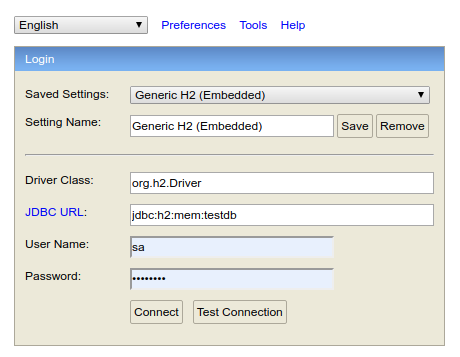
\includegraphics[width=\pictureWidth cm]{Bilder/Kapitel_5/h2_login.png}
\caption{Login der \textit{H2}-Console\label{fig:h2_login}}
\end{figure}

Der Login erfolgt über den Nutzernamen und das Passwort, die in der \textit{application-dev.properties}-Datei hinterlegt wurden. Nach dem Login wird dann ein Textfeld angezeigt, in dem \ac{SQL}-Satements auf alle in der linken Seite der Oberfläche angezeigten Tabellen ausgeführt werden können.

\subsubsection{Microservice Kommunikation}

Anders als im \textit{prod}-Modus einer Anwendung, können alle Teile der Anwendungen, darunter auch die Microservices, individuell gestartet werden. Dabei sind keine weiteren Services nötig, alle Abhängigkeiten werden in der Test Umgebung simuliert. Somit müssen bei Abhängigkeiten zwischen den Microservices keine anderen Services gestartet werden. Da dies in einer Microservice Architektur im allgemeinen nicht vorgesehen ist, sind hierbei vor allem das \ac{API}-Gateway und der \textit{Eureka}-Server zu betrachten. In der Entwicklungsumgebung muss zuerst der \textit{Eureka}-Server gestartet werden, worauf das \ac{API}-Gateway sich dann bei seinem Start beim \textit{Eureka}-Server registrieren kann. Danach können alle anderen Services gestartet werden. Im \textit{dev}-Modus ist das nicht der Fall, hier sind Gateway- und Service-Discovery-Funktionen deaktiviert. Dies geschieht über Konfigurationen in der \textit{application-dev.properties}-Datei, die benötigten Eigenschaften sehen wie folgt aus:

\newpage
\begin{lstlisting}[caption={Discovery und Gateway Deaktivierung}]
eureka.client.enabled=false
eureka.client.register-with-eureka=false
\end{lstlisting}


\subsubsection{Start der Anwendung}

Der wohl gravierendste Unterschied zwischen der produktiven und der Entwicklungsumgebung liegt im Start der Anwendung. Möchte man einen Teil der Anwendung starten, um ihn in der \textit{dev}-Umgebung zu testen, so benötigt man dazu, wie bereits erwähnt, keine Instanzen des \textit{Eureka}-Servers oder des \ac{API}-Gateways. Man stößt lediglich die Kompilierung und den Build-Prozess des Services an und startet die danach generierte \textit{*.jar}-Anwendung mit dem Konsolenbefehl \textsc{java -jar [dateiname].jar}.\\
\linebreak
Um dies Prozesse jedoch nicht manuell anstoßen zu müssen sind die im Kapitel \ref{sec:entwicklungsumgebung} beschriebenen Tools hilfreich. Durch die \ac{IDE} kann der Programmcode automatisch kompiliert, gebuilded und gestartet werden. Das alles sogar im sogenannten \textit{Debug}-Modus der \ac{IDE}, welcher es ermöglicht, Breakpoints im Code zu setzen, bei deren Durchlaufen das Programm gestoppt wird, um die Variablen während der Laufzeit auslesen zu können. In der in dieser Praxisarbeit empfohlenen \ac{IDE} sind die Buttons zum Start und zum Debuggen der Anwendung rechts oben in der Oberfläche zu finden. Diese sehen wie folgt aus:

\begin{figure}[H]
\centering

\includegraphics[width=\pictureWidth cm]{Bilder/Kapitel_5/ide_start_prog.png}
\caption{Start und Debuggen der Anwendung in der \ac{IDE}\label{fig:ide_start_prog}}
\end{figure}

Der Linke der markierten Buttons ist zum Start der Anwendung im normalen Modus zuständig. Dabei ist kein Debugging möglich, es werden beim Ausführen der Anwendung jedoch auch weniger Ressourcen des Systems benötigt. Der Rechte der beiden Buttons ist der Debug Button. Durch diesen können im Code Breakpoints gesetzt werden, die die Anwendung auch stoppen. Dieser Modus benötigt jedoch mehr Systemressourcen. Anzumerken ist ebenfalls, das beide Modi das erwähnte Hot-Deployment aus Kapitel \ref{sec:hot_deploy} unterstützen. 

\subsubsection*{Einrichtung des \textit{dev}-Modus}

Die \ac{IDE} \textit{IntelliJ IDEA} erleichtert es ungemein, eine Einstellung für die Entwicklung im \textit{dev}-Modus zu erstellen. Hierfür öffnet man lediglich das im rechten oberen Bildrand befindliche Dropdown und wählt \textit{Edit Configurations...} aus. Danach erscheint folgendes Menü:

\begin{figure}[H]
\centering
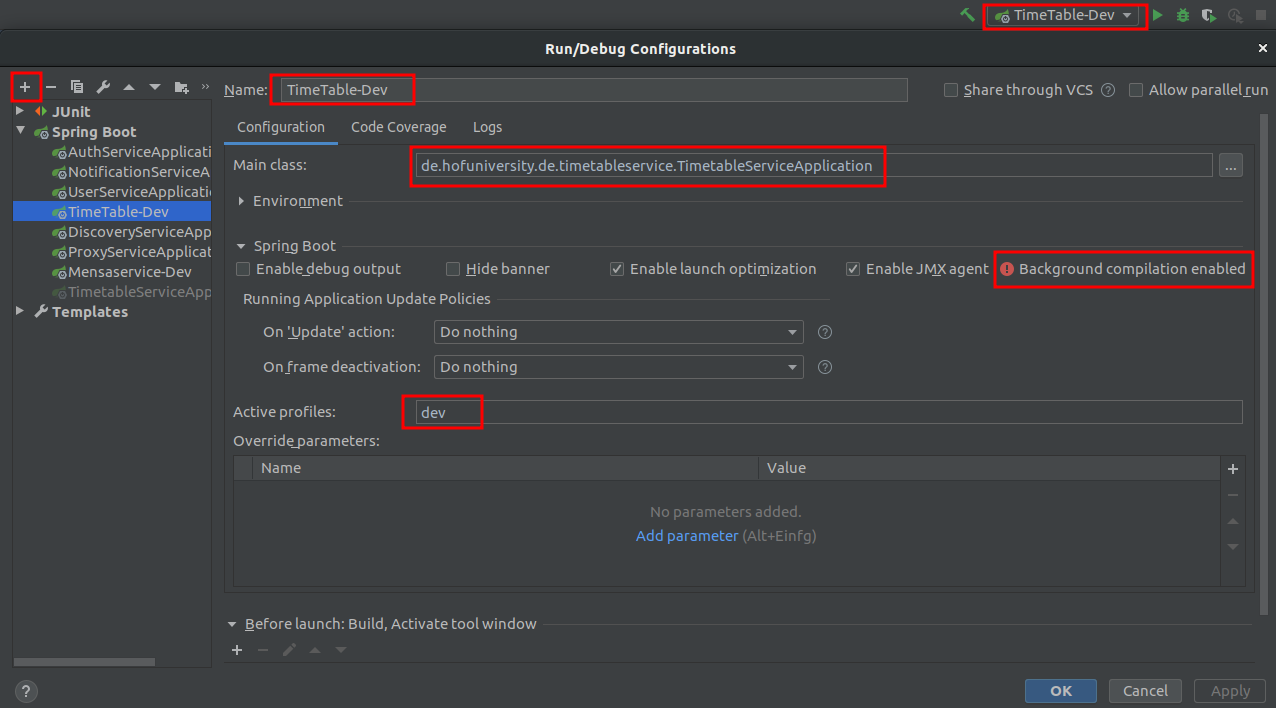
\includegraphics[width=\pictureWidth cm + 2 cm]{Bilder/Kapitel_5/ide_dev_config.png}
\caption{Einstellen der Test-Umgebung in der \ac{IDE}\label{fig:ide_dev_config}}
\end{figure}

Die in der Abbildung \ref{fig:ide_dev_config} markierten Felder werden nun von oben nach unten und von links nach rechts erläutert:

\begin{itemize}
\item Auswählen von \textit{Edit Configurations...} im Dropdown
\item Erstellen einer neuen \textit{Spring} Konfiguration
\item Vergeben eines Namens für die Konfiguration
\item \textit{! Background compilation enabled} sollte angezeigt werden, da dies in der Einrichtung zum Hot-Deployment in Kapitel \ref{sec:hot_deploy} eingerichtet wurde. 
\item Zuordnung zum \textit{Active Profile} \textsc{dev} (Der Name ist hier frei wählbar, wird aber später gebraucht)
\end{itemize}

Zusätzlich muss nun in den Ressourcen des Microservices eine neue Properties-Datei erstellt werden, die nach folgendem Schema benannt werden muss:\\
\textit{application-}\textsc{dev}\textit{.properties}\\
\textsc{dev} ist hierbei der Name des \textit{Active Profile}, welches vorher konfiguriert wurde. In diesem Properties-File können nun alle Konfigurationen für die Testumgebung hinterlegt werden, die \textit{dev}-Konfiguration, die in der \ac{IDE} vorgenommen wurde, lädt diese dank der Namensgebung automatisch. Das Properties-File hat den selben Aufbau und Zweck wie das in Kapitel \ref{sec:resources} erklärte File.

\section{Prod-Environment}

Das starten der Services auf der produktiven Umgebung bedarf einer festgelegten Vorgehensweise. Hierbei ist die Reihenfolge der Schritte, die im folgenden kurz aufgelistet werden, kritisch.

\begin{enumerate}
\item Start des \textit{Eureka}-Servers
\item Start des \ac{API}-Gateways
\item Start der anderen Services
\end{enumerate}

Das Starten der Services erfolgt nach dem Erstellen der einzelnen \textit{*.jar}-Dateien für jeden Service. Diese werden dann mit folgendem Befehl gestartet:

\begin{lstlisting}[caption={Starten eines \textit{jar}-Files}]
~: java -jar [dateiname].jar
\end{lstlisting}

Da die Reihenfolge dieses Vorgangs kritisch ist und beliebig viele Services gestartet werden können, bietet sich es an, diesen Vorgang per Skript zu automatisieren. In diesem Zug kann man auf die Ausgabe der Programme in eine Log-Datei weiterleiten und die Anwendung im Allgemeinen beobachten. Ein passendes Skript auf einer UNIX-basierten Umgebung könnte wie folgt aussehen:

\newpage
\begin{lstlisting}[caption={Skript zum Verwalten der Microservices}]
#!/bin/sh
#repeat each step per *.jar files 
#needed in correct order

#Start API packaged in microservice.jar
start(){
    #Create .log directory
    mkdir .log > /dev/null 2>&1
    echo "Starting API on port 8080"
    #Start timetableAPI.jar, Redirect Error and Output to logfile
    java -jar ~/microservice.jar >> ~/.log/microservice.log 2>&1 &
    echo "Started API"
}

#Stop API Process running on tcp port 8080
stop(){
    echo "Stopping API on port 8080"
    #fuser finds processfile, -k kills process
    fuser -k 8080/tcp
    echo "Stopped API"
}

#Checking status of API running on tcp port 8080
status(){
    #if fuser finds process for port 8080
    if fuser 8080/tcp then
        echo "API running on port 8080"
    else
        echo "API not running"
    fi
}

restart(){
    echo "Stopping API to reload"
    stop
    start
    echo "Successfully restarted API"
}

#Switch params to call functions
case $1 in
start)
    start
;;
stop)
    stop
;;
status)
    status
;;
restart|reload)
    restart
;;
*)
    echo "Usage: $0 (start|stop|status|restart|reload)"
    exit 1
esac

#End script
exit 0
\end{lstlisting}